\documentclass{scrartcl}
\usepackage[utf8]{inputenc}
\usepackage[german]{babel}
\usepackage{amsmath}
\usepackage{natbib}
\usepackage{graphicx}
\usepackage{float}
\floatplacement{figure}{htbp}
\floatplacement{table}{htbp}
\usepackage[
  section, % Floats innerhalb der Section halten
  below,   % unterhalb der Section aber auf der selben Seite ist ok
]{placeins}
\usepackage{subcaption}
\usepackage{xfrac}


\begin{document}

\section*{Übungsblatt 2 -- Cerberus}

    \subsection*{Aufgabe 1}

        Im Folgenden soll das $512 \times 512$ Bild aus Abbildung \ref{fig:bild} mithilfe der Singulärwertzerlegung
        \begin{equation*}
            \mathbf{A} = \mathbf{U} \cdot \mathbf{\Sigma} \cdot \mathbf{V}^{\text{T}}
        \end{equation*}
        und der Rang-\textit{k}-Approximation komprimiert werden.
        %\begin{figure}
        %    \centering
        %    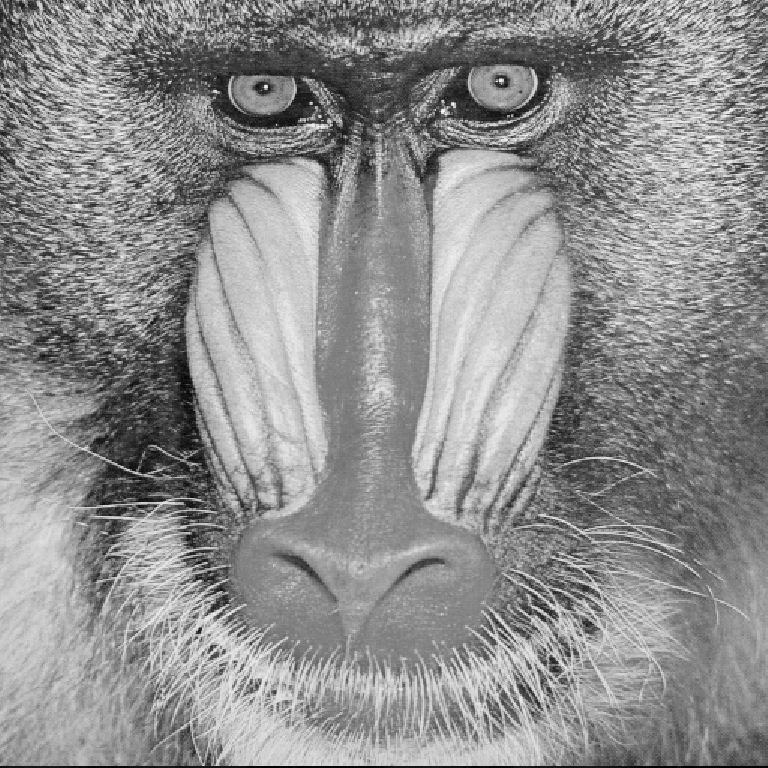
\includegraphics[width=0.5\textwidth]{A1/build/bild.pdf}
        %    \caption{Originalbild.}
        %    \label{fig:bild}
        %\end{figure}
        Die Rekonstruktion und Approximation erfolgt mithilfe von 
        \begin{equation*}
            \mathbf{\tilde{A}} = \sum_{i = 1}^{k} \sigma_i \vec{u}_i \vec{v}_i^{\text{T}} \:\:\: \text{mit} \: k \leq 512.
        \end{equation*}
        \begin{center}
            \tiny{$\sigma_i \: \hat{=}$ i-tes Diagonalelement von $\mathbf{\Sigma}$, $\vec{u}_i \: \hat{=}$ i-ter Spaltenvektor von $\mathbf{U}$,
                  $\vec{v}_i \: \hat{=}$ i-iter Spaltenvektor von $\mathbf{V}$.}
        \end{center}
        Die approximierten Bilder für $k = 10, 20, 50$ befinden sich in Abbildung \ref{fig:approx}.
        \begin{figure}
            \centering
            \begin{subfigure}[b]{0.3\textwidth}
                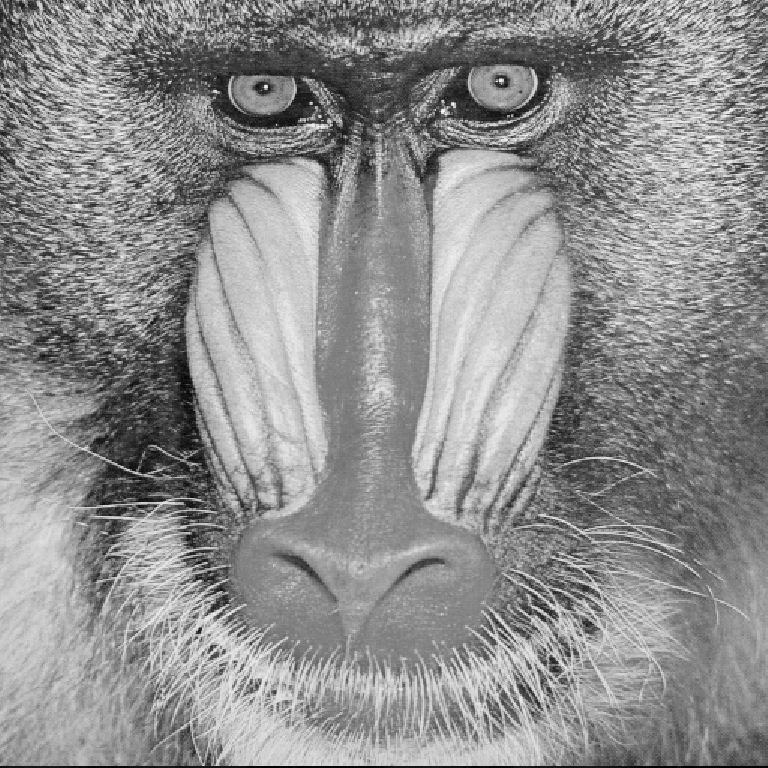
\includegraphics[width=\textwidth]{A1/build/bild.pdf}
                \caption{Originalbild.}
                \label{fig:bild}
            \end{subfigure}
            ~ %add desired spacing between images, e. g. ~, \quad, \qquad, \hfill etc. 
            %(or a blank line to force the subfigure onto a new line)
            \begin{subfigure}[b]{0.3\textwidth}
                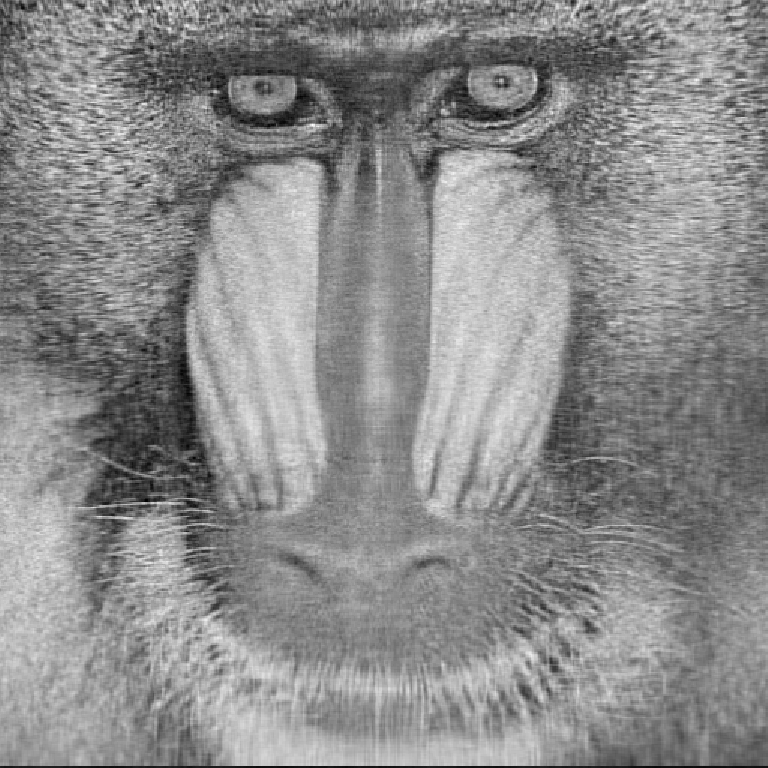
\includegraphics[width=\textwidth]{A1/build/A50.pdf}
                \caption{$k=50$.}
                \label{fig:A50}
            \end{subfigure}
            
             %add desired spacing between images, e. g. ~, \quad, \qquad, \hfill etc. 
              %(or a blank line to force the subfigure onto a new line)
            \begin{subfigure}[b]{0.3\textwidth}
                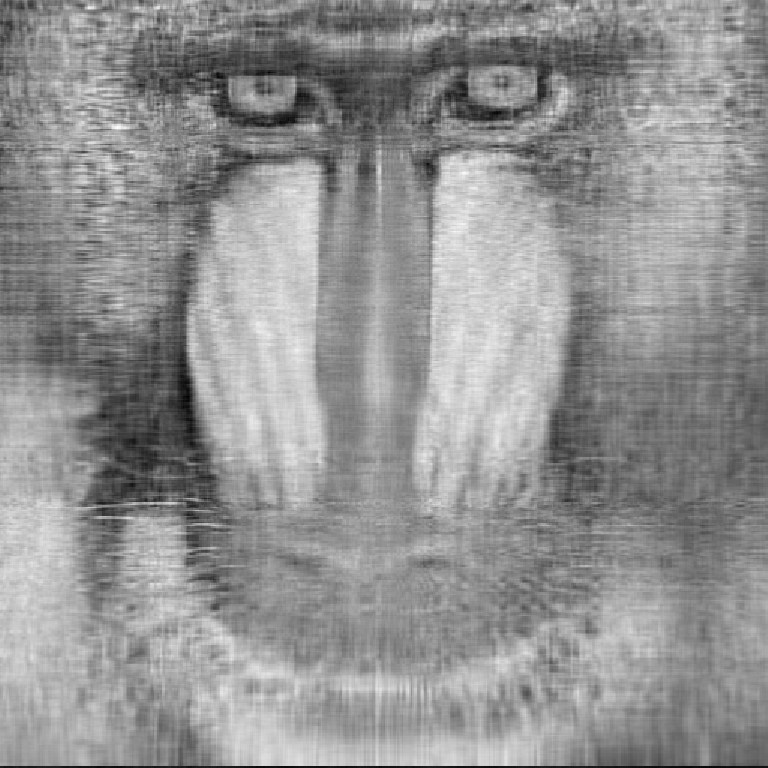
\includegraphics[width=\textwidth]{A1/build/A20.pdf}
                \caption{$k=20$.}
                \label{fig:A20}
            \end{subfigure}
            ~
            \begin{subfigure}[b]{0.3\textwidth}
                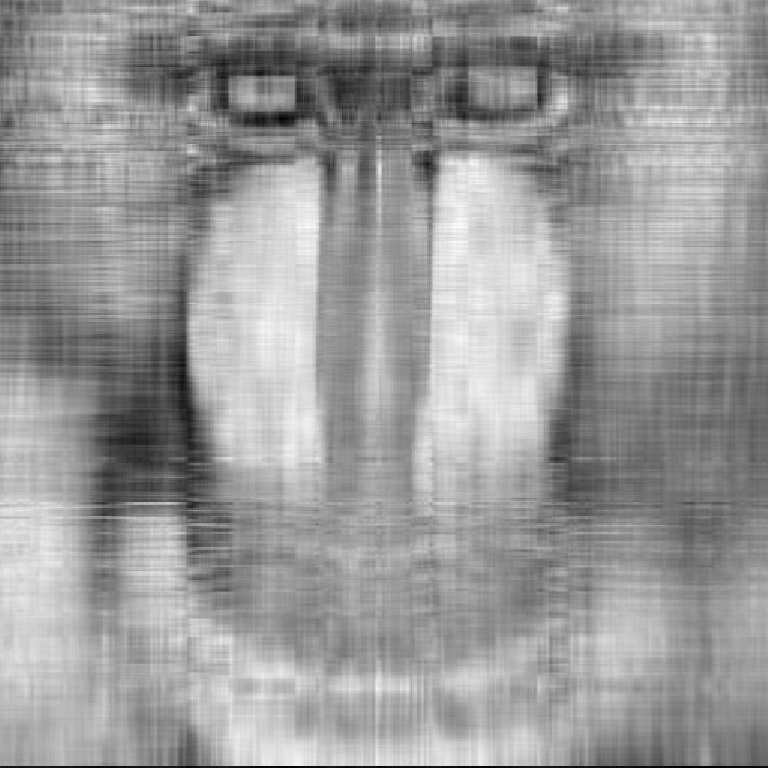
\includegraphics[width=\textwidth]{A1/build/A10.pdf}
                \caption{$k=10$.}
                \label{fig:A10}
            \end{subfigure}
            \caption{Approximation von Abbildung \ref{fig:bild} für verschiedene $k$.}\label{fig:approx}
        \end{figure}
        Die SVD scheint sich gut zur Kompression zu eignen, da sich das Bild, wie in Abbildung \ref{fig:A50} zu sehen, mit nur knapp
        $10 \, \%$ der Singulärwerte schon sehr gut rekonstruieren lässt. Selbst bei einer so extremen Kompression wie in Abbildung
        \ref{fig:A10} ist das Motiv noch ganz grob zu erkennen.
        

\end{document}
